%\documentclass[a4paper,12pt,twocolumn,dvipdfmx,Flow]{jsarticle}
\documentclass[a4j,12pt,dvipdfmx]{jsarticle}
%\AtBeginDvi{\special{pdf:mapfile sotsuron.map}}
\RequirePackage{fix-cm}
\usepackage[top=35mm,bottom=30mm,left=30mm,right=20mm]{geometry}
\usepackage[dvipdfmx]{graphicx}
\usepackage{comment}
\usepackage{tikz}
\usepackage{here}
\usepackage{array,booktabs}
\usepackage{listings,jlisting}
\usepackage{rawfonts,flow}
%\usepackage{pxchfon}
\usepackage{color}
\usepackage{jtygm}

%\setminchofont{ipam.ttf}
%\setgothicfont{ipag.ttf}
%\setminchofont{TanukiMagic.ttf}
%\setgothicfont{TanukiMagic.ttf}

\makeatletter
\g@addto@macro\@floatboxreset\centering
\makeatother

\lstset{%
  language={C},
  basicstyle={\small},%
  identifierstyle={\small},%
  commentstyle={\small\itshape},%
  keywordstyle={\small\bfseries},%
  ndkeywordstyle={\small},%
  stringstyle={\small\ttfamily},
  frame={tb},
  breaklines=true,
  columns=[l]{fullflexible},%
  numbers=left,%
  xrightmargin=0zw,%
  xleftmargin=3zw,%
  numberstyle={\scriptsize},%
  stepnumber=1,
  numbersep=1zw,%
  lineskip=-0.5ex,%
  tabsize=2%
}
\renewcommand{\lstlistingname}{Code}% Listing -> Algorithm
\renewcommand{\figurename}{Fig}% Listing -> Algorithm
\renewcommand{\tablename}{Table}% Listing -> Algorithm
\renewcommand{\abstractname}{\flushleft\textbf{\fontsize{12pt}{30pt}\selectfont Abstract}\hfill}

\usetikzlibrary{patterns}

\newcommand{\Dt}{\Delta t}
\newcommand{\II}{I\hspace{-.1em}I}
\newcommand{\maru}[1]{\ooalign{
\hfil\resizebox{.8\width}{\height}{#1}\hfil
\crcr
\raise.1ex\hbox{\large$\bigcirc$}}}
\newcommand*\circled[1]{\tikz[baseline=(char.base)]{
  \node[shape=circle,draw,inner sep=2pt] (char) {#1};}}

\title{二値化画像処理による \\ 粉粒体高速流動の画像情報の統計的処理}
%Comparative evaluation of autocorrelation function of time-dependent configuration of particulate/powdery systems in fast translational motion and the velocity of the apparent motion of them
\author{吉渡 匠汰}
\date{ } %change

%\setlength{\textwidth}{155truemm}
%\setlength{\fullwidth}{\textwidth}
%\setlength{\oddsidemargin}{37truemm}
%\addtolength{\oddsidemargin}{-1truein}
%\setlength{\topmargin}{30truemm}
%\setlength{\textheight}{237truemm}
%\addtolength{\topmargin}{-1truein}

\begin{document}
%\onecolumn{

%\maketitle
\begin{center}
\fontsize{22pt}{30pt}\selectfont
\textcolor{white}{卒業研究報告書}

卒\quad 業\quad 研\quad 究\quad 報\quad 告\quad 書
\\[7pt]
\fontsize{20pt}{30pt}\selectfont
\hrulefill \\
\begin{flushleft}
課題タイトル

二値化画像処理による粉粒体高速流動の\\ 画像情報の統計的処理
\\[14pt]
tochastic characterization method \\
for motion pictures \\
of flowing powdery or granular matters \\
By vision binarization 
\\[7pt]
\end{flushleft}
\hrulefill
\\[15pt]
平成28年度

\fontsize{18pt}{20pt}\selectfont
\begin{flushleft}
福島工業高等専門学校
\end{flushleft}

学科名 物質工学科 42番 吉渡匠汰
%
%\textcolor{white}{学科名 物質工学科 42}番\textcolor{white}{ 吉渡匠汰}
%
%\textcolor{white}{学科名 物質工学科 42}番\textcolor{white}{ 吉渡匠汰}
\\[36pt]
指導教員  車田研一  \circled{{\large 印}}
\end{center}

\clearpage

%\twocolumn[
\clearpage
\fontsize{12pt}{15pt}\selectfont
\begin{abstract}
\fontsize{12pt}{15pt}\selectfont
The texture is great importance to the sense of sight. But we can't explain simply the texture. So it is considered to "{\it tacit dimension}, Michael Polany". In recent years, however, analysis of short time have become possible with high-speed camera. Thus, this field came to study. Analysis was done hitherto by sight\cite{sight1} \cite{sight2}. In this study, I analyze the motion of spheres, powders and liquid by binarization-centered image processing to detect the location and size of the particle and calculate autocorrelation functions meaning the time-shift degree of similarity of the change of position . I compare functions and motion to connect them.  \par
The most importance factor is the time which the value decline and remainin value\cite{first}. They depend on the particle size. On top of that, one particle is like another particle that the diameter is neary. In conclusion, we recognize this extremely short time to differentiate kind of particles or liquid. In particular, powders appearing like liquid have shorter decline time like water. On balance, analysis of the motion to caliculate autocorrelation function is avaiable to digitize the texture. 
\end{abstract}
%}
%]

\clearpage

%\twocolumn[
\tableofcontents
%]

\clearpage

\section{物体流動の解析法}
%\lstinputlisting[caption=hoge,label=hoge]{"test.txt"}
\begin{comment}
\scriptsize
\STRUCT{struct name}{structure purpose}{%
	\ACTION{init}%
	\IF{if\\ to test}%
	\THEN{%
		\ACTION{action}%
	}%
	\ELSE{%
		\ACTION{action2}%
	}%
	\ENDIF%
}%
\normalsize
\end{comment}
全く別の印象を受ける球と粉、水の運動(流動)の相違点の1つとして定常性の差が挙げられる。定常性は映像をタイムシフトさせたときにどれくらい整合性があるかという尺度に等しい。これを自己相関関数として計算することにより解析を行った。
\subsection{画像処理について}
物体の動きを正確に追うため本研究では二値化画像処理を用いている。二値化とは各画素について一定の閾値以下ならば白、そうでないならば黒にするという処理を施し、二色の画像を作成する処理である。運動する対象の色とギャップの大きい色を背景にして撮影し、二値化処理によって対象を白または黒で抜き出すことができる。 \par
二値化処理を施した画像の例としてFig\ref{fig:threshold}を示す。
\begin{figure}[H]
	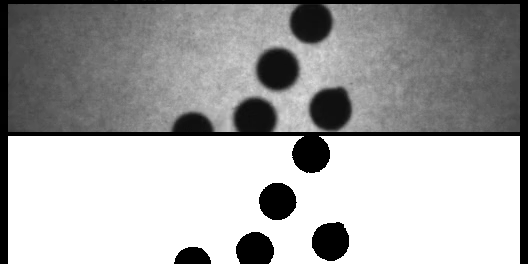
\includegraphics[clip,width=7.0cm]{bb_image.png}
	\caption{二値化画像の例 上:撮影された映像の1フレーム、下:二値化画像}
	\label{fig:threshold}
\end{figure}
本研究では解析の開発も行った。用いた言語はC++とPythonである。画像処理に関わるソースコードをCode \ref{code:two}に示す。画像処理にはOpenCVライブラリを用いている。Code \ref{code:two}は粉粒体の落下運動の動画からフレームを切り抜き、トリミングおよび二値化処理を行うプログラムである。そして、トリミング画像・二値化画像・2つを並べた画像の3種類を各フレームごとにナンバリングして保存する。二値化を行うthreshold関数は閾値を引数に持つ(ここでは33となっている)。これはピクセルを黒に変換する境界で、閾値を低くすればするほど二値化画像は黒の割合が高くなる。
\lstinputlisting[caption=動画のフレーム切り抜きと二値化,label={code:two},language=Python]{"getimage.py"}
\subsection{相関関数の評価方法}
%まず画像間の類似性というものを考える。ここで類似性とは同一時系列上にある2つの画像がどれだけ似ているかという意味で用いているが、まずは類似性の数値化を試みた。そのためには類似性の具体的な定義を行う必要がある。本研究では次のように定義した、「画像間で色が一致しているピクセルの数[px]」。イメージ画像をFig\ref{fig:exfall}に示す。比較する際にまずベースフレーム($t_0$時点)を一つ決める。次に$t_0+\Delta t$後の画像と比較する。色が一致するピクセル数を$S(\Delta t)$と表すことにする。$S(0)$は同じ画像同士の比較なので完全に一致するため、$S(0)$は比較画像のピクセル数に等しい。$\Delta t$が少しずれて、例えば$S(\frac{1}{5000})$のようになると$S(0)$よりも少し小さくなる。これを$0 \leq \Delta t \leq 0.1 [s]$の範囲で計算する。なお落下運動は定常なものであるため、$t_0$を適当に20点選び平均をとっている。 \par
前述したように自己相関関数とは映像の定常性を表す尺度である。1変数関数$f(t)$には一つのtに対して1つの値が対応するのに対し、映像には1つの画像(フレーム)が対応する。1変数関数の整合性を求めるとき、元信号の値とタイムシフト後の信号の値を比べることになる。この考えを映像に拡張する。すなわち元映像のある時間の画像とタイムシフト後の同じ時間の画像を比較し、その類似性を計算ればよい。画像の類似性は2つの画像をピクセル単位で見たときに色が一致しているピクセルが何個あるかという指標で表せる。精度を考えれば元信号と重なっている範囲全てを網羅すべきであるが、画像処理は重い処理なため元信号から適当な20点を選び、タイムシフトは0〜0.1秒に限定している。
\begin{comment}
\begin{equation}
	\cos (\vec{q} ,\vec{d}) = \frac{\vec{q} ・ \vec{d}}{|\vec{q}| ・ |\vec{d}|}
\end{equation}
\end{comment}
$S(0 \leq \Delta t \leq 0.1)をS(0)$の値で割り、規格化した値を自己相関関数$G(\Delta t)$とする。$S(\Delta t)の範囲が0 \leq S(\Delta t) \leq S(0)であるから、相関関数G(\Delta t)の値域は0 \leq G(\Delta t) \leq 1となる$。
\begin{figure}[hbtp]
	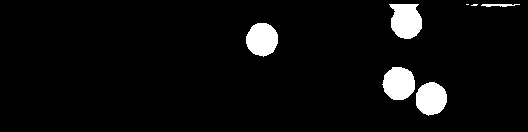
\includegraphics[clip,width=7.0cm]{0.png}
	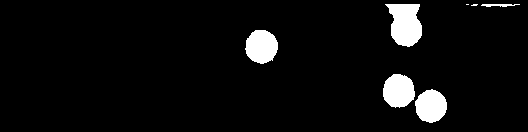
\includegraphics[clip,width=7.0cm]{3.png}
	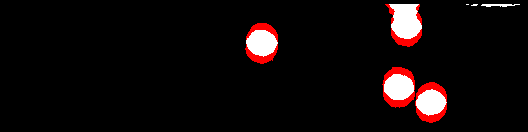
\includegraphics[clip,width=7.0cm]{0and3.png}
	\caption{画像比較のイメージ(上:t=0s,中央:$\frac{3}{5000}s$,下:比較) \newline $黒、白 \cdots 色が一致 ,赤 \cdots 色が不一致$}
	\label{fig:exfall}
\end{figure}
自己相関関数を計算するために2つのプログラムを作成した。まず、このプログラム群を以下に示す。
Code \ref{code:txt}は二値化画像を元にテキストファイルを作成するプログラムである。このプログラムは解析上必須ではないが、画像ファイルへのアクセスは時間がかかるプロセスなため一旦テキストに書き出すことで今後の解析時間の短縮を行っている。なお、二値化画像は0:黒、255:白の2種類のピクセルで構成されている。テキスト化に当たってはファイルの可読性を考慮して1:白に変換している。
\lstinputlisting[caption=二値化画像のテキスト書き出し,label={code:txt},language=C++]{"getbw.cpp"}
Code \ref{code:count}はCode \ref{code:txt}によって作成されたテキストファイルを元にして重複ピクセルをカウント、自己相関関数の計算を行うプログラムである。ベースフレームと比較するフレームの各ピクセル情報を比較し一致すればカウントを+1するといった処理を行っている。基準とするベースフレームの数は20個、1つのベースフレームに対して501フレーム(0.1秒間分)の比較を行っている。保存する値は比較するフレーム数と同じ501個である。つまり、1回目のベースフレームとの比較により501個分のカウント($S(\Dt):S(0)〜S(500)$)ができるが、2回目以降はこのカウントに累積させていくことになる。
全てのフレームについて比較とカウントを行った後に正規化処理を行っている。正規化時点で1つのカウントには比較20回分の値が保存されている。これら501個分のカウントをベースフレーム同士の比較$S(0)$で除する。これにより$S(0)=1$以降1以下の値が500個続く。これらの値を自己相関関数として出力する。
\lstinputlisting[caption=重複ピクセルカウント,label={code:count},language=Python]{"andbw.py"}
\begin{figure}
%\begin{flushleft}
\begin{tabular}{cc}
\begin{minipage}[t]{0.45\hsize}
\scriptsize
\setiftext{yes}{no}
\STRUCT{andbw}{自己相関関数を求めるアルゴリズム}{%
    \ACTION{c[t:0-500]=all0}%
    \ACTION{i=0}%
	\REPEAT{%
      \ACTION{t=0}%
	  \ACTION{ベースフレーム(0+i*30.png)を習得}%
	  \ACTION{i++}%
	  \REPEAT{%
	    \ACTION{比較フレーム(i+t.png)と比較\\(右参照)}%
	  }%
      \ACTION{t++}%
	  \UNTIL{$t \geq 500$}%
	}%
	\UNTIL{$i > 20$}%
	\ACTION{cを規格化}%
}%
\normalsize
%\end{flushleft}
\end{minipage}&
\begin{minipage}[t]{0.45\hsize}
%\begin{comment}
%\begin{flushright}
\scriptsize
\setiftext{yes}{no}
\STRUCT{andbw}{ピクセルをカウントするアルゴリズム}{%
  \ACTION{j=0}%
  \REPEAT{%
    \ACTION{j番目のピクセル同士を比較}%
	\IF{色が一致}%
      \THEN{%
        \ACTION{c[t]++}%
      }%
      \ELSE{%
      }%
    \ENDIF%
	\ACTION{j++}%
  }%
  \UNTIL{全てのピクセルについて探査終了}%
}%
\normalsize
%\end{flushright}
%\end{comment}
\end{minipage}
\end{tabular}
\label{fig:auto_flow}
\caption{自己相関計算プログラムのフローチャート}
\end{figure}

\section{実験と結果}
\subsection{撮影環境}
測定に用いるのは落下装置とハイスピードカメラである。落下装置はダンボール箱を加工したもので、光を通したり撮影したりするための穴や物体を充填する漏斗とストッパーで構成されている。装置とカメラの距離は70 cmとし、カメラに映っている範囲で物体の落下速度は約2 m/sとなるようにしている。また、カメラのシャッタースピードは5000 fps($\frac{1}{5000}秒に1回$)、露光時間は$\frac{1}{80000}秒$である。 \par
本研究においてほとんどの物体は黒背景にして白色で抜き出している。これは物体にライトを当てることによって物体が白っぽく映るためであるが、金属球については反射によって色のむらができてしまうため、白背景にして後ろから光を当てることにより黒で抜き出している。
\subsection{物体の種類}
本研究で測定した物体はTable\ref{tb:ballkind}に示す7種類である。 \\
\begin{table}[H]
	\caption{実験に使用した物体 \label{tb:ballkind}}
	\begin{tabular}{lr}
		\toprule
		種類 & 直径[mm] \\
		\midrule
		金属球 & 6.2 \\
		BB弾 & 6.0 \\
		発泡ポリスチレン & 1.54 \\
		砂(15〜20メッシュ) & 1 \\
		砂(20〜30メッシュ) & 0.7 \\
		海砂(150〜200メッシュ) & 0.08 \\
		ガラスビーズ & 0.02-0.08 \\
		水(白絵の具で着色) & - \\
		\bottomrule
	\end{tabular}
\end{table}

Table\ref{tb:ballkind}で金属球、BB弾、発泡ポリスチレンは実際に測定したものだが、砂と海砂については表記されたメッシュ値を参考におおよその直径を決めている。 \par

\subsection{事故相関関数}
実験で得られた各物体の相関関数を下記にまとめる。なお、グラフ中の略称についてはTable\ref{tb:ballname}を参照のこと。また、Fig\ref{fig:overall}に0.1秒間の自己相関関数の変化を示す。 \par
\begin{table}[H]
	\caption{粉粒体の略称 \label{tb:ballname}}
	\begin{tabular}{lr}
		\toprule
		種類 & 略称 \\
		\midrule
		金属球 & Metal \\
		BB弾 & BB \\
		発泡ポリスチレン & EPS \\
		砂(15〜20メッシュ) & sand1520 \\
		砂(20〜30メッシュ) & sand2030 \\
		海砂(150〜200メッシュ) & seasand \\
		ガラスビーズ & glass \\
		水(白絵の具で着色) & water \\
		\bottomrule
	\end{tabular}
\end{table}
自己相関関数は総じてはじめに減少し、その後傾きが小さくなり場合によってはほぼ一定の値を保っていることがわかる。 \par
\begin{figure}[H]
	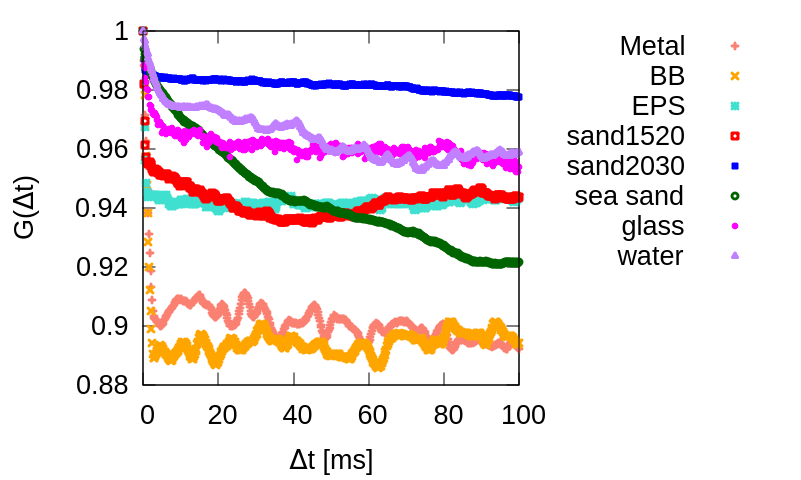
\includegraphics[scale=0.4]{multi.png}
	\caption{各物体の相関関数}
	\label{fig:overall}
\end{figure}
$0 \leq \Delta t \leq 4 [ms]$を拡大したグラフがFig\ref{fig:init}である。このグラフの結果から各粉粒体を3つのグループに分類した。第1グループは粒径6 mmを超えるものである。金属球(Metal)とBB弾(BB)がこれに当たる。グループ1はFig\ref{fig:init}の範囲において2つの期間に分かれている。1つは$0 \leq \Dt \leq 2.5$にある相関が減少する区間である。これを区間Iと呼ぶ。もう1つはほぼ相関が一定になる区間\II である。2つの区間には明確な境界があり、2.5〜2.8 msと見られる。また区間\II については他のグループよりも振動が大きい。振動が大きい理由としては球が離散体として運動するため、確率的にベースフレームとほとんど一致しないフレームがあるからである。 \par
これよりも小さく粒径1 mm以上のものをグループ2とする。発泡ポリスチレン(EPS)と砂15-20メッシュ(sand1520)が含まれる。このグループについてもグループ1と同様2つの区間が見られるが、区間Iの時間がグループ1よりも短くなっている。境界は1 msあたりである。 \par
最後に残りをグループ3とする。これらは粒径が1 mmに満たない粒もしくは液体である。グループ3は特に海砂以下については区間Iが消失しているように見える。砂(20-30メッシュ)に関しては0.5 ms付近に境界があることが確認できるので、境界が見られない粉粒体については、より短い間隔で撮影を行うことで区間Iを発見することができると思われる。\par
区間Iと区間\II の境界を「相関持続時間$t_c$」とする。目視の範囲でわかる$t_c$をTable\ref{tb:tc_eye}にまとめる。
\begin{figure}[H]
	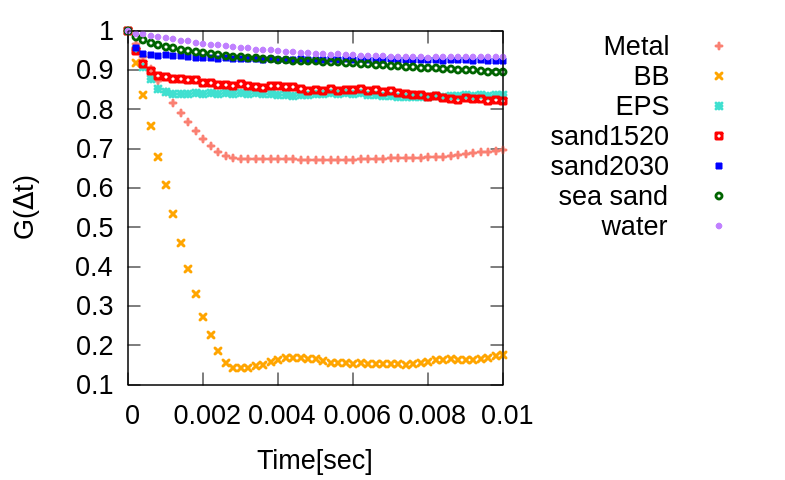
\includegraphics[scale=0.4]{init.png}
	\caption{各物体の相関関数(0.004秒まで)}
	\label{fig:init}
\end{figure}

\begin{table}[H]
	\caption{相関持続時間(目視) \label{tb:tc_eye}}
	\begin{tabular}{lr}
		\toprule
		グループ & $t_c [ms]$ \\
		\midrule
		グループ1 & 2.5-2.8 \\
		グループ2 & 1 \\
		グループ3(砂(20-30メッシュ)) & 0.5 \\
		グループ3(その他) & - \\
		\bottomrule
	\end{tabular}
\end{table}

\subsection{微分を用いた相関持続時間$t_c$の算出}
前述したように相関持続時間$t_c$は目視により大体の検討をつけることができるが、軸の縮尺等によって見え方は変わってくる。そこで、見た目という定性的な分析法ではなく、微分を用いて定量的に$t_c$を求めた。Fig\ref{fig:diff}は自己相関関数を時間差で微分したグラフである。 \par
自己相関関数は区間Iでは負の傾きを持つが、区間\II は0に近い傾きで振動する。そのため微分$\frac{dG(\Dt)}{d\Dt}$で0付近になるときの時間差$\Dt がt_c$と一致すると考えられる。
\begin{figure}[H]
	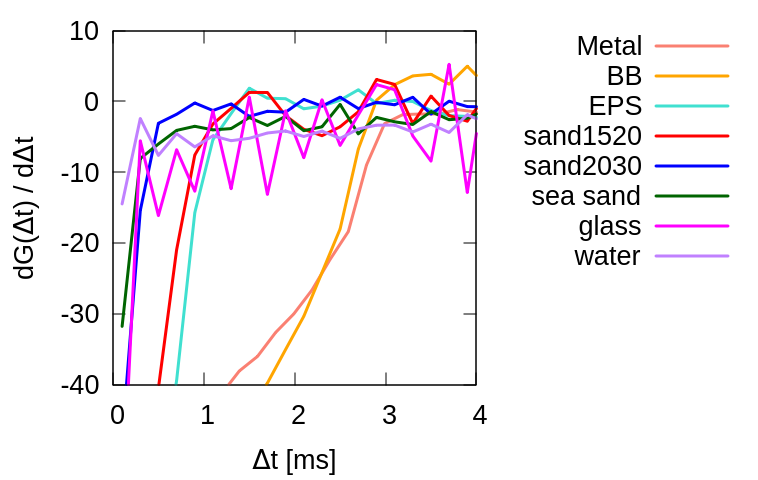
\includegraphics[scale=0.4]{diff.png}
	\caption{各物体の相関関数の微分}
	\label{fig:diff}
\end{figure}
微分を用いる場合、傾きが-10になるときの$\Dt$を調べることで目視とおおよそ一致することがわかった。Table\ref{tb:tc_diff}に各グループの微分値が-10になるおおよその時間を示す。
\begin{table}[H]
	\caption{相関持続時間 \label{tb:tc_diff}}
	\begin{tabular}{lrr}
		\toprule
		%グループ & $t_c [ms](微分)$ & $t_c [ms](目視)$ \\
		グループ & $t_c [ms](微分)$  \\
		\midrule
		%グループ1 & 2.7 & 2.5-2.8 \\
		%グループ2 & 0.8 & 1 \\
		%グループ3(砂(20-30メッシュ)) & 0.4 & 0.5 \\
		%グループ3(その他) & 0.2 & - \\
		グループ1 & 2.7  \\
		グループ2 & 0.8  \\
		グループ3(砂(20-30メッシュ)) & 0.4  \\
		グループ3(その他) & 0.2 \\
		\bottomrule
	\end{tabular}
\end{table}

\subsection{グループ1の比較}
グループ1は相関減少区間(区間I)と一定になる区間(区間\II )が明確に分かれていることが特徴である。グループ1の自己相関関数をFig\ref{fig:one}に示す。グループ1に属する金属球(Metal, 6.2 mm)とBB弾(BB, 6.0 mm )で大きな差はみられない。これは粒径のさがあまりないためであると考えられる。測定した粉粒体の種類が少ないので完全に傾向を予想することはできないが、自己相関関数の概形は粒径にのみに影響され、種類にはよらないものと思われる。
\begin{figure}[H]
	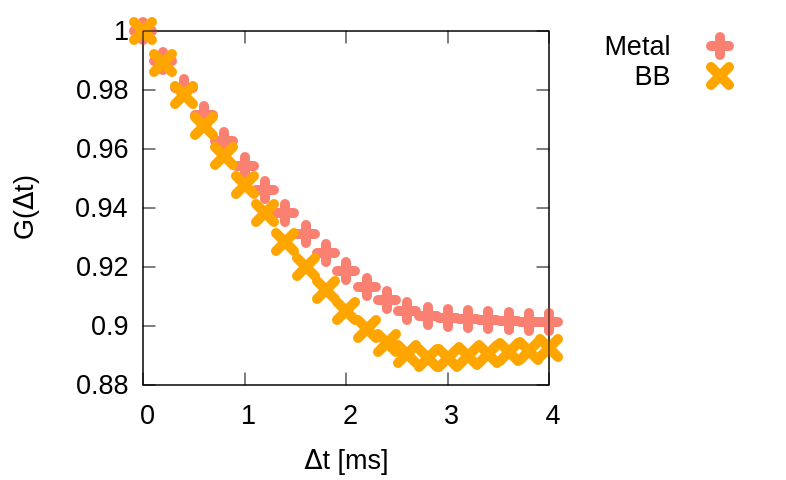
\includegraphics[scale=0.4]{one.png}
	\caption{グループ1の自己相関関数}
	\label{fig:one}
\end{figure}
\subsection{グループ2の比較}
グループ2の発泡ポリスチレンと砂(15-20メッシュ)は微分後の形を見ても明らかなように粒径が細かい砂の方が相関減少時間が短い。その結果砂のほうが区間\II の値は大きい。このグループのように落下粉粒体を連続体として捉えることができる場合、相関減少は連続体の帯のヘリとその周辺の変化を表している。すなわち相関減少がより少ない砂は発泡ポリスチレンよりもヘリの変化が少ないということが言える。
\begin{figure}[H]
	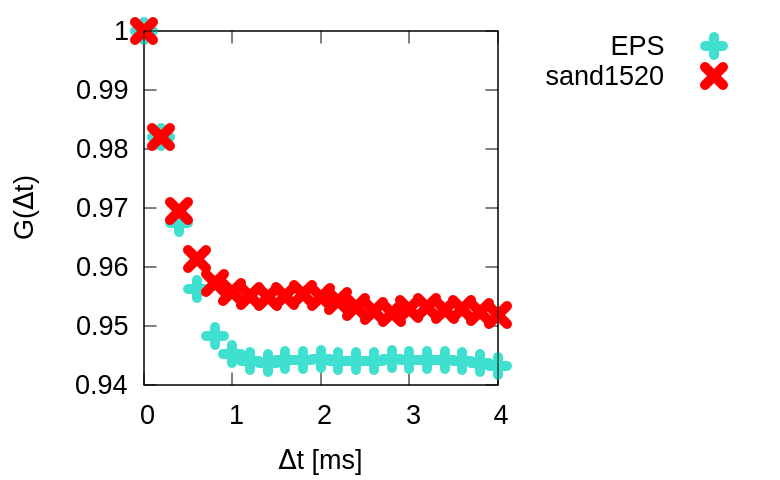
\includegraphics[scale=0.4]{two_big.png}
	\caption{グループ2の自己相関関数}
	\label{fig:two}
\end{figure}
\subsection{グループ3の比較}
グループ3の自己相関関数の形はそれぞれ特徴のある形をしている。まず、砂(20-30メッシュ)はグループ1,2の傾向を引き継ぎ、相関減少時間を0.5 msと短くし、以降相関をほぼ一定に保っている。この砂(20-30メッシュ)までが区間分けができる粒径となる。その次に細かい海砂には区間\II が見られず、100 ms, G=0.92まで緩やかに減少を続けている。また、60 ms付近でグループ2の相関を追い抜いている。ただし減少速度は8つの中でも小さいため4 msという短い間隔で見ればグループ3として分類できる。ガラスビーズや水の相関には再び2つの区間が現れる。しかも5~6 msというグループ1よりも長い時間減少時間を持つ。ガラスビーズと水についても海砂と同じく相関は0.95以上という高い値を保っている。
\begin{figure}[H]
	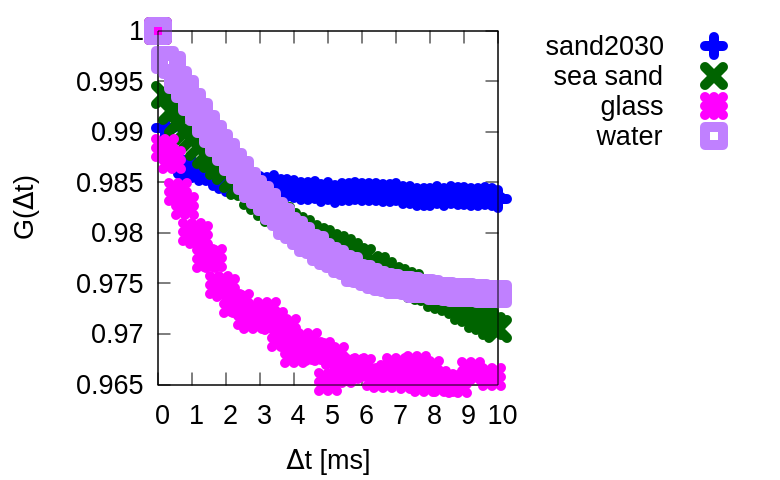
\includegraphics[scale=0.4]{three_up.png}
	\caption{グループ3の自己相関関数}
	\label{fig:three}
\end{figure}
\subsection{球(離散体)と粉(連続体)の相関減少の相違}
グループ3における相関減少時間と相関減少速度から海砂以下について次の予測が立てられる。粒径がある程度小さくなると相関減少時間は長くなるということである。そもそもグループ1に代表される離散体の相関減少区間は、初期位置からの球1つ分の移動を表していた。それがグループ2で少し意味が変わり、粒径が細かくなると映像に帯、すなわち連続体の部分が現れる。連続体部分の相関減少はヘリの小さな変化に起因している。つまりグループ2の相関減少は離散体と連続体両方の要素を含んでいる。さらにグループ3には変化の小さい連続体のみが写っているため、相関減少速度も小さくなる。そのためグループ1よりも減少時間が長くなるものと考えられる。ただし減少が緩やかな分減少量は小さく、保持される相関値が高くなるため、区間\II との区別がつきづらくなる。本研究では、減少量が小さいためこの相関減少は無視し、相関減少時間が0.5 ms以下で曖昧または消失したグループ3としてまとめている。
\section{透明な物体の測定}
\subsection{透明な球・液体の解析方法}
自己相関関数の計算には二値化画像処理が不可欠である。二値化する条件は被写体と背景の色のギャップが大きいことである。しかし、透明な物体は背景を透過するため二値化に十分なギャップを作ることができない。そこで、別な方法により二値化に似た処理を提案する。 \par
今回注目したのは透明な物体が背景を透過するとき、完全に背景を映し出さないという性質である。つまり透明な物体であっても多くの場合背景が歪んで見え、その物体を認識することができる。これを利用して背景の歪みを検出するプログラムを作成した。この測定法には背景に方眼紙(Fig\ref{fig:block})を用いる。
\begin{figure}[H]
	\centering
	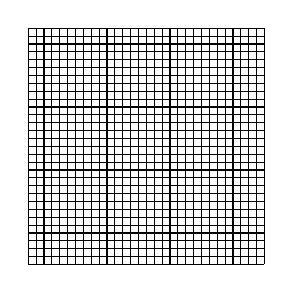
\begin{tikzpicture}
		\draw[step = 1 mm] (0,3) grid (3,0);
	\end{tikzpicture}
	\caption{背景(1 mm方眼)}
	\label{fig:block}
\end{figure}
Fig\ref{fig:block}を背景にし、透明な物体を落下運動させる。この映像を二値化し、線分を検出する。この段階では背景や光の反射によって物体の色が安定しない。だが、物体がない場所はそのまま線が映っているため線が検出できるが、物体がある場所は線が見えなくなるため検出できなくなる。次に真っ白で大きさが映像のものと同じ画像を用意する。これに線分を検出した場所に沿って太い線を引く。すると背景部分の多くが黒く塗りつぶされるため擬似的に透明物体を白く抜き出すことができる。Fig\ref{fig:line}に透明物体の落下画像(初期二値化済み)と疑似二値化画像を示す。
\begin{figure}[H]
	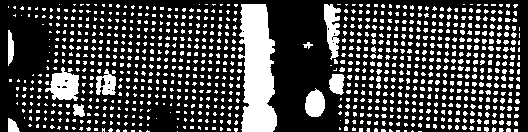
\includegraphics[scale=0.4]{water_two.png}
	
\includegraphics[scale=0.4]{water_line.png}
	\caption{落下映像(上)と疑似二値化画像(下)}
	\label{fig:line}
\end{figure}
Code \ref{code:line}に線分検出プログラムを示す。本プログラムは疑似二値化画像の作成を目的としている。関数getlineが実際に線分を検出している。getlineではまず対象画像を読み込んだ後、白色画像を作成している。次に線分をHough変換によって検出している。これにより線分の場所や長さを座標という形で得ることができる。この座標を元に白色画像に検出した線分の位置をなぞるように線分を描画する。この線分の太さを適当に太くすると線分の位置周辺が黒く塗りつぶされる。これを検出した線分全てに行う。線分が見えている周辺は透明物体が通っていない=背景なので、最終的に背景のおおよそが黒く塗りつぶされることになる。
\lstinputlisting[caption=線分検出,label={code:line},language=C++]{"cruz.cpp"}
\subsection{結果}
結果をFig \ref{fig:compare}に示す。図は絵の具で着色した水を通常の方法で解析したものと線分を検出することによって解析したものの比較である。線分の方法だと全体的に相関が小さく算出される。これは線分を完全に検出できず、背景であっても白い部分があるからである。$G(0)=1$は共通なので、直後に急激な相関減少が現れている。着色したものでは6 ms以降で相関減少が落ち着くが、線分検出の方はばらつきが大きく、評価は難しい。それでも4 ms以降は比較的落ち着きが見えるため、ある程度は解析ができているものと思われる。
\begin{figure}[H]
	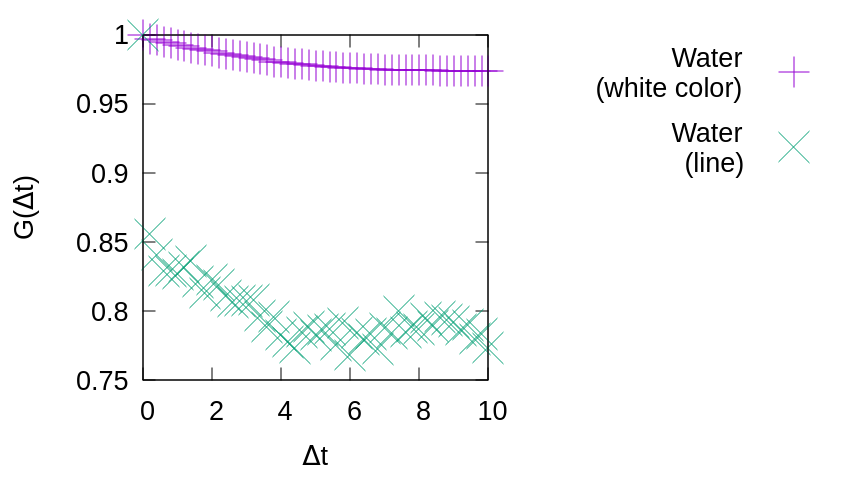
\includegraphics[scale=0.4]{compareline.png}
	\caption{線分検出法}
	\label{fig:compare}
\end{figure}
\section{結論}
二値化を用いて流動映像を解析し、自己相関関数を求めることで粒径と流動の外観に関係性があることがわかった。粒径が細かいほど映像の定常性は高くなり、連続体として観測される。また、細かい粉体の流動映像は数値から見ても液体のものと酷似しており、これが見分けがつきにくい要因となっている。しかし、液体は相関の減少が他の粉体よりも緩やかであるため、その僅かな時間の違いから両者を見分けることができる場合もあると考えられる。

\begin{thebibliography}{3}
  \bibitem{sight1} Patrick Cavanagh, “Visual cognition”, {\it Vision Research}, {\bf 51}, 2011, 1538-1551
  \bibitem{sight2} 車田,梅本,大槻,『顕著に運動する粒状体群の特徴づけへの「仮現運動(apparent motion)」の試行的応用』,公益社団法人化学工学会第 48 回秋季大会(徳島大学),2016/9/8
  \bibitem{first} 車田,『粉粒体のながれのうねり(時間的ゆらぎ)をとらえる ―シャッフリング画像処理による流動体の構造相関持続時間スケールの把捉の試み―』北関東地区化学技術懇話会技術サロン 「動く・流れる・感じる」化学工学部門依頼講義,宇都宮大学,2016/12/9
\end{thebibliography}
\end{document}
